\documentclass[a4paper,12pt]{article} % тип документа

% Поля страниц
\usepackage[left=2.5cm,right=2.5cm,
    top=2cm,bottom=2cm,bindingoffset=0cm]{geometry}
    
%Пакет дял таблиц   
\usepackage{multirow} 
    
%Отступ после заголовка    
\usepackage{indentfirst}


% Рисунки
\usepackage{floatrow,graphicx,calc}
\usepackage{wrapfig}

%%% Работа с картинками
\usepackage{graphicx}  % Для вставки рисунков
\graphicspath{{images/}{images2/}}  % папки с картинками
\setlength\fboxsep{3pt} % Отступ рамки \fbox{} от рисунка
\setlength\fboxrule{1pt} % Толщина линий рамки \fbox{}
\usepackage{wrapfig} % Обтекание рисунков и таблиц текстом

% Создаёем новый разделитель
\DeclareFloatSeparators{mysep}{\hspace{1cm}}

% Ссылки?
\usepackage{hyperref}
\usepackage[rgb]{xcolor}
\hypersetup{				% Гиперссылки
    colorlinks=true,       	% false: ссылки в рамках
	urlcolor=blue          % на URL
}


%  Русский язык
\usepackage[T2A]{fontenc}			% кодировка
\usepackage[utf8]{inputenc}			% кодировка исходного текста
\usepackage[english,russian]{babel}	% локализация и переносы




% Математика
\usepackage{amsmath,amsfonts,amssymb,amsthm,mathtools}

%%% Дополнительная работа с математикой
\usepackage{amsmath,amsfonts,amssymb,amsthm,mathtools} % AMS
\usepackage{icomma} % "Умная" запятая: $0,2$ --- число, $0, 2$ --- перечисление


% Что-то 
\usepackage{wasysym}


\begin{document}
\begin{center}
	\footnotesize{ФЕДЕРАЛЬНОЕ ГОСУДАРСТВЕННОЕ АВТОНОМНОЕ ОБРАЗОВАТЕЛЬНОЕ 			УЧРЕЖДЕНИЕ ВЫСШЕГО ОБРАЗОВАНИЯ}\\
	\footnotesize{МОСКОВСКИЙ ФИЗИКО-ТЕХНИЧЕСКИЙ ИНСТИТУТ\\(НАЦИОНАЛЬНЫЙ 			ИССЛЕДОВАТЕЛЬСКИЙ УНИВЕРСИТЕТ)}\\
	\footnotesize{ФАКУЛЬТЕТ ОБЩЕЙ И ПРИКЛАДНОЙ ФИЗИКИ\\}
	\hfill \break
	\hfill \break
	\hfill \break
	\hfill \break
\end{center}


\begin{figure*}[h]
    \centering
    \includegraphics*[width=10cm,height=7cm,keepaspectratio]{mipt_eng_text_png.png}
    \label{fig:my_label}
\end{figure*}


\begin{center}   
    \hfill \break
	\hfill \break
	\hfill \break
	\large{Лабораторная работа № 4.3.3\\ \hfill \break\Large{Исследование разрешающей способности микроскопа методом Аббе}}\\
	\hfill \break
	\hfill \break
	\hfill \break
	\hfill \break
	\begin{flushright}
		Баранов Даниил\\
		Группа Б02-103
	\end{flushright}
	\hfill \break
	\hfill \break
\end{center}
\hfill \break
\hfill \break
\hfill \break
\hfill \break
\begin{center}
	Долгопрудный, 2023 г.
\end{center}
\thispagestyle{empty}

\newpage

\textbf{Цель работы:} определение дифракционного предела разрешения объектива микроскопа методом Аббе.

\textbf{В работе используется:} лазер; кассета с набором сеток разного периода; линзы; щель с микрометрическим винтом; оптический стол c набором рейтеров и крепёжных винтов; экран; линейка.

\section{Теоретическая справка}

Всякая оптическая система, предназначенная для получения изображений, имеет конечный предел разрешения, т. е. ограниченную возможность раздельного наблюдения близко расположенных предметов. Принципиальной причиной, ограничивающей предел разрешения, является дифракция световых волн. Разрешающей способностью оптического прибора называют минимальное расстояние $l_{min}$ между двумя точками в пространстве предметов, которое прибор может разрешить. При визуальном наблюдении изображения в качестве критерия разрешения применяют так называемый критерий Рэлея.

Для иммерсионного микроскопа (объект находится в иммерсионной среде -- жидкости с показателем преломления n) разрешающая способность объектива при некогерентном освещении

\begin{equation*}
    l_{min}\approx\frac{0,61\lambda}{n sin A},
\end{equation*}
где $A$ — апертурный угол объектива микроскопа (см. рис. \ref{ust}), т. е. угол между оптической осью и лучом, направленным из центра объекта в край линзы.

Рассмотрим теперь когерентно освещённый объект, наблюдаемый в микроскоп. Схема образования изображения в объективе микроскопа представлена на рис. \ref{ust}. Для простоты рассмотрим случай, когда предметом является периодическая структура (дифракционная решётка), освещаемая параллельным пучком лучей. При наблюдении в микроскоп предмет располагается вблизи переднего фокуса объектива. При освещении решётки волнами, наклонными к оси, с углом наклона чуть меньшим апертуры $A$ волны нулевого порядка сфокусируются на край диафрагмы. Для получения изображения достаточно, чтобы на противоположные края сфокусировались волны 1-го порядка, т. е. угол между волнами 0 и 1 порядка должен быть равен $2A$. Минимальное разрешаемое объективом расстояние определяется условием

\begin{equation}
    l_{min} \approx\frac{\lambda}{sinA} \approx\frac{\lambda}{D/2f},
    \label{diaf}
\end{equation}
где $D$ — диаметр диафрагмы. При этом диафрагма, расположенная симметрично, пропускает нулевой и $\pm 1$ дифракционные максимумы.

\begin{figure}[H]
    \centering
    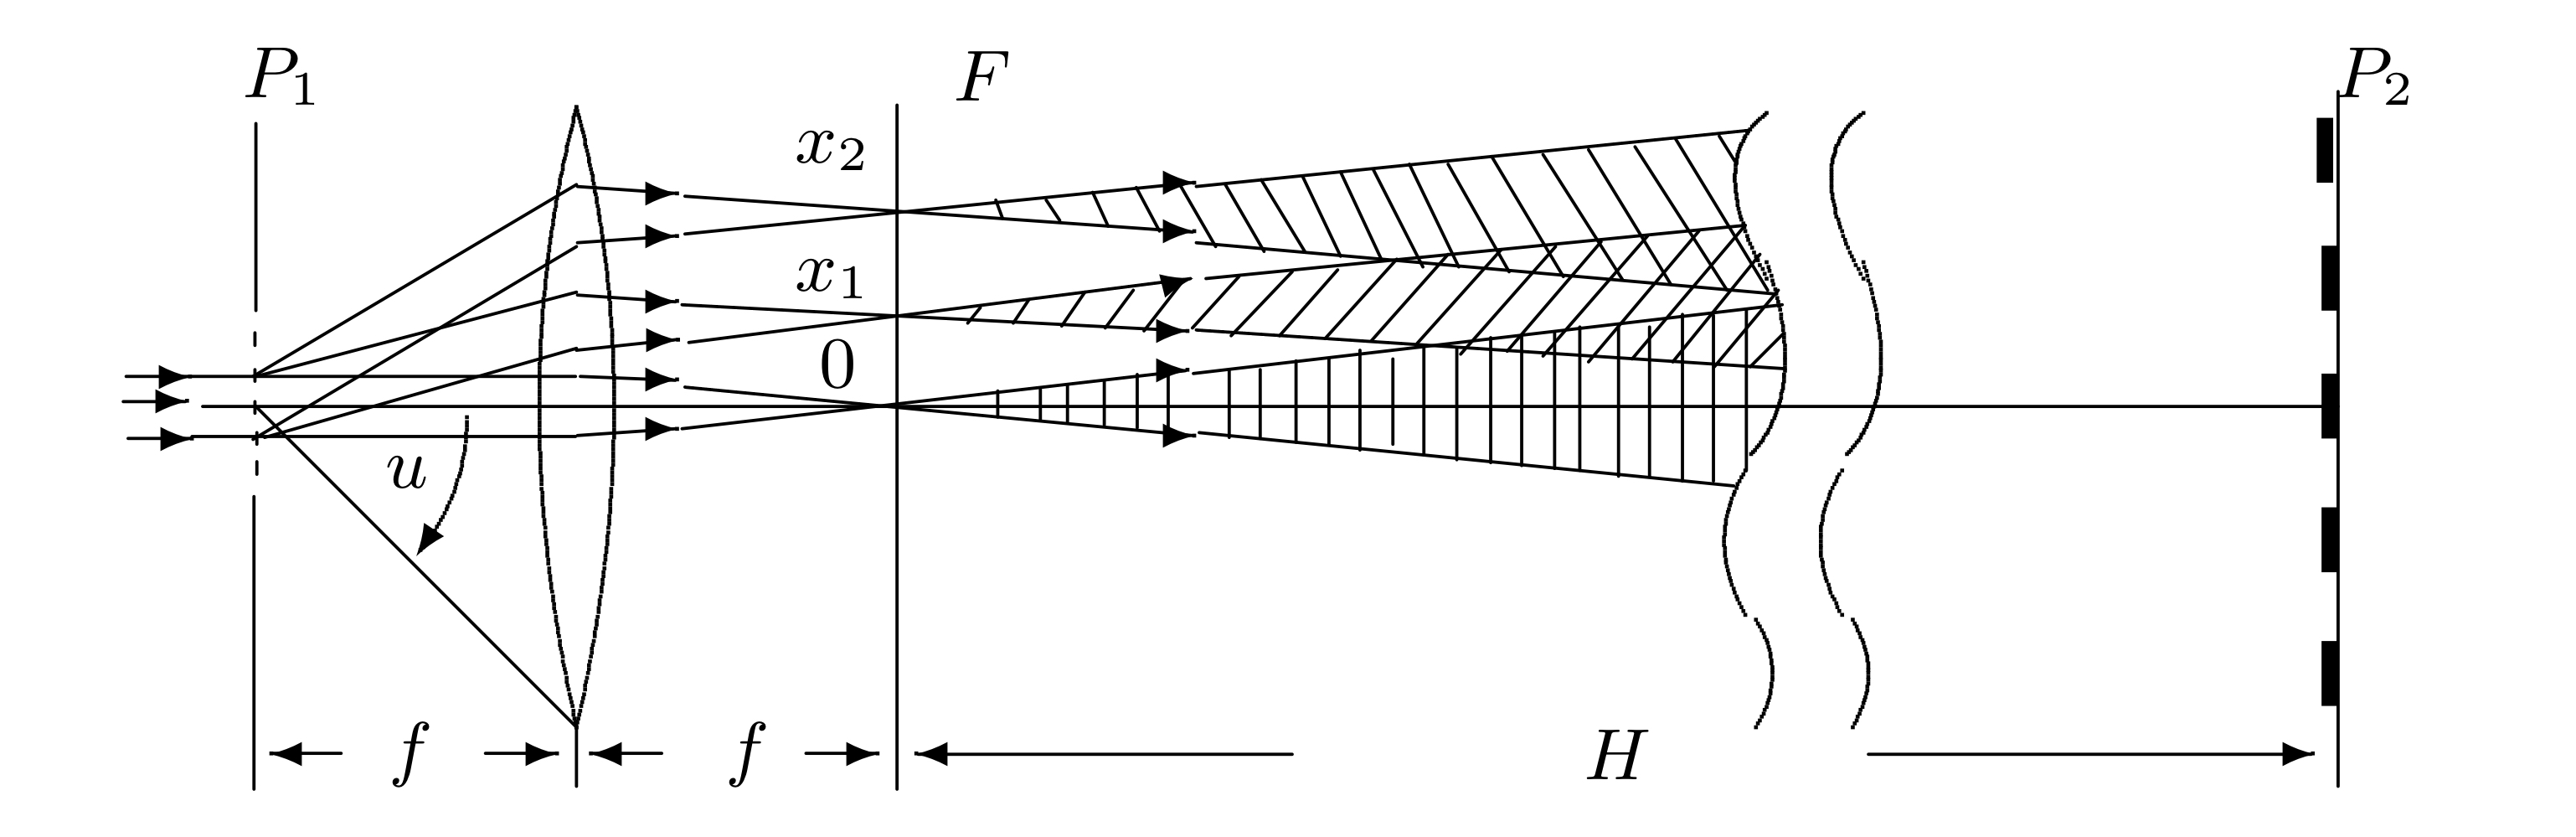
\includegraphics[scale=0.14]{4.3.3/ust.jpeg}
    \caption{\centering Образование изображения в объективе микроскопа. $P_1$ — плоскость предмета, $F$ — задняя фокальная плоскость объектива, $P_2$ — плоскость, сопряжённая с предметной плоскостью. В плоскости $P_2$ световые пучки сильно перекрываются
}
    \label{ust}
\end{figure}

В нашей работе применяется двумерная решётка -- сетка. Её можно рассматривать как две скрещенные (перпендикулярные друг к другу) решётки. Узкий пучок монохроматического света, пройдя через решётку с вертикальными штрихами, даёт совокупность максимумов, расположенных вдоль горизонтальной линии. Световой пучок, соответствующий каждому максимуму, проходя через вторую решётку, распадается на новую совокупность световых пучков, дающих максимумы вдоль вертикальной линии. Главные максимумы возникают тогда, когда одновременно выполняются условия:

\begin{equation}
    dsin\theta_x = m_x\lambda,\  \  dsin\theta_y=m_y\lambda
\end{equation}
где $m_x$ и $m_y$ — целые числа, характеризующие порядки дифракцион- ных максимумов, $\theta_x$ и $\theta_y$ — направления на главные дифракционные максимумы в горизонтальной и вертикальной плоскостях соответственно.

\begin{figure}[H]
    \centering
    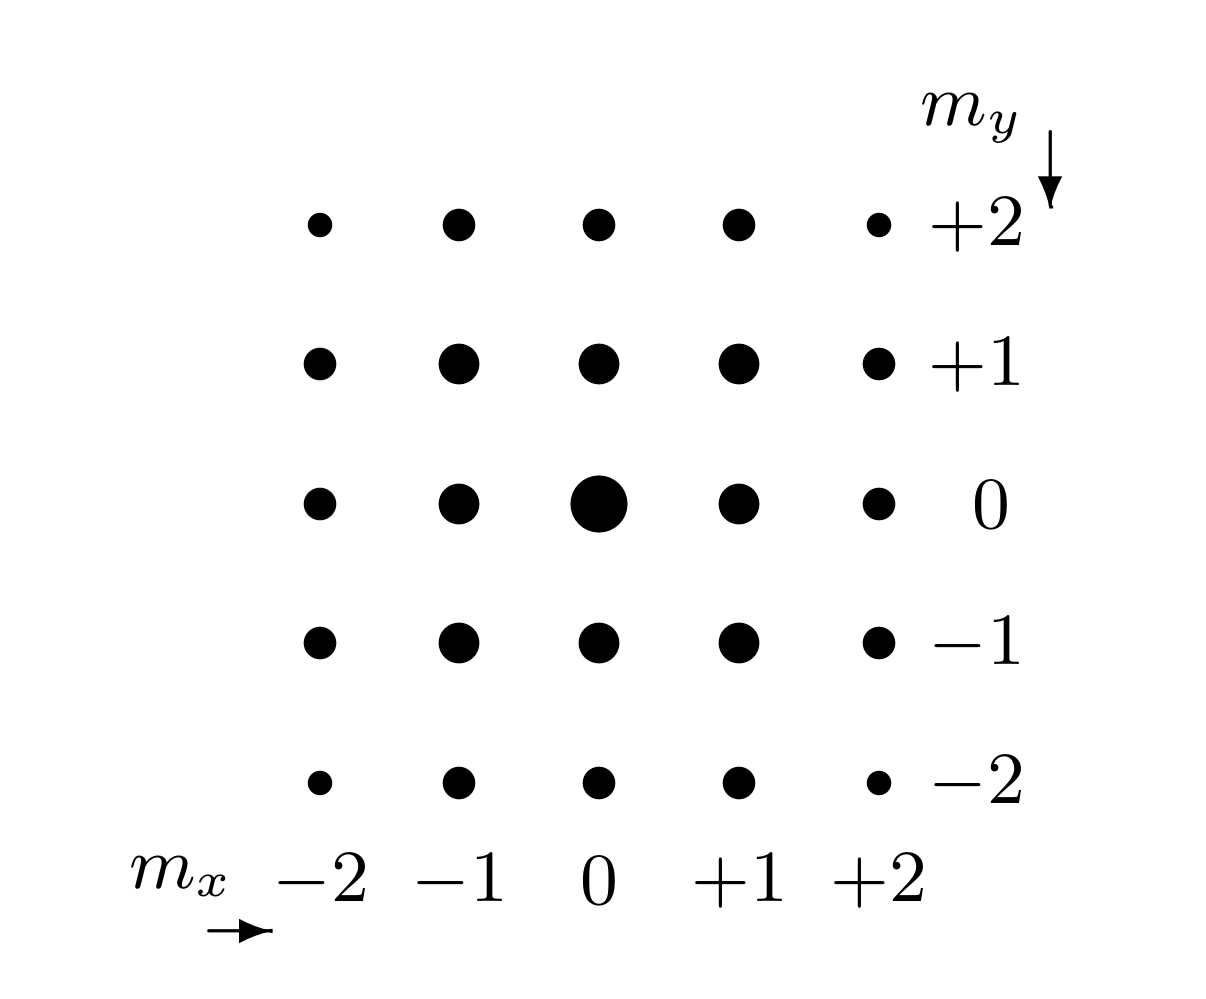
\includegraphics[scale=0.2]{4.3.3/max.jpeg}
    \caption{\centering Дифракция Фраунгофера на двумерной решётке (сетке). Максимумы изображены кружками, размеры которых характеризуют интенсивности}
    \label{max}
\end{figure}

\section{Экспериментальная установка}

Схема модели проекционного микроскопа приведена на рис. \ref{micro}. Предметом служат сетки, расположенные в кассете. Смена сеток осуществляется поворотом внешнего кольца кассеты.

\begin{figure}[H]
    \centering
    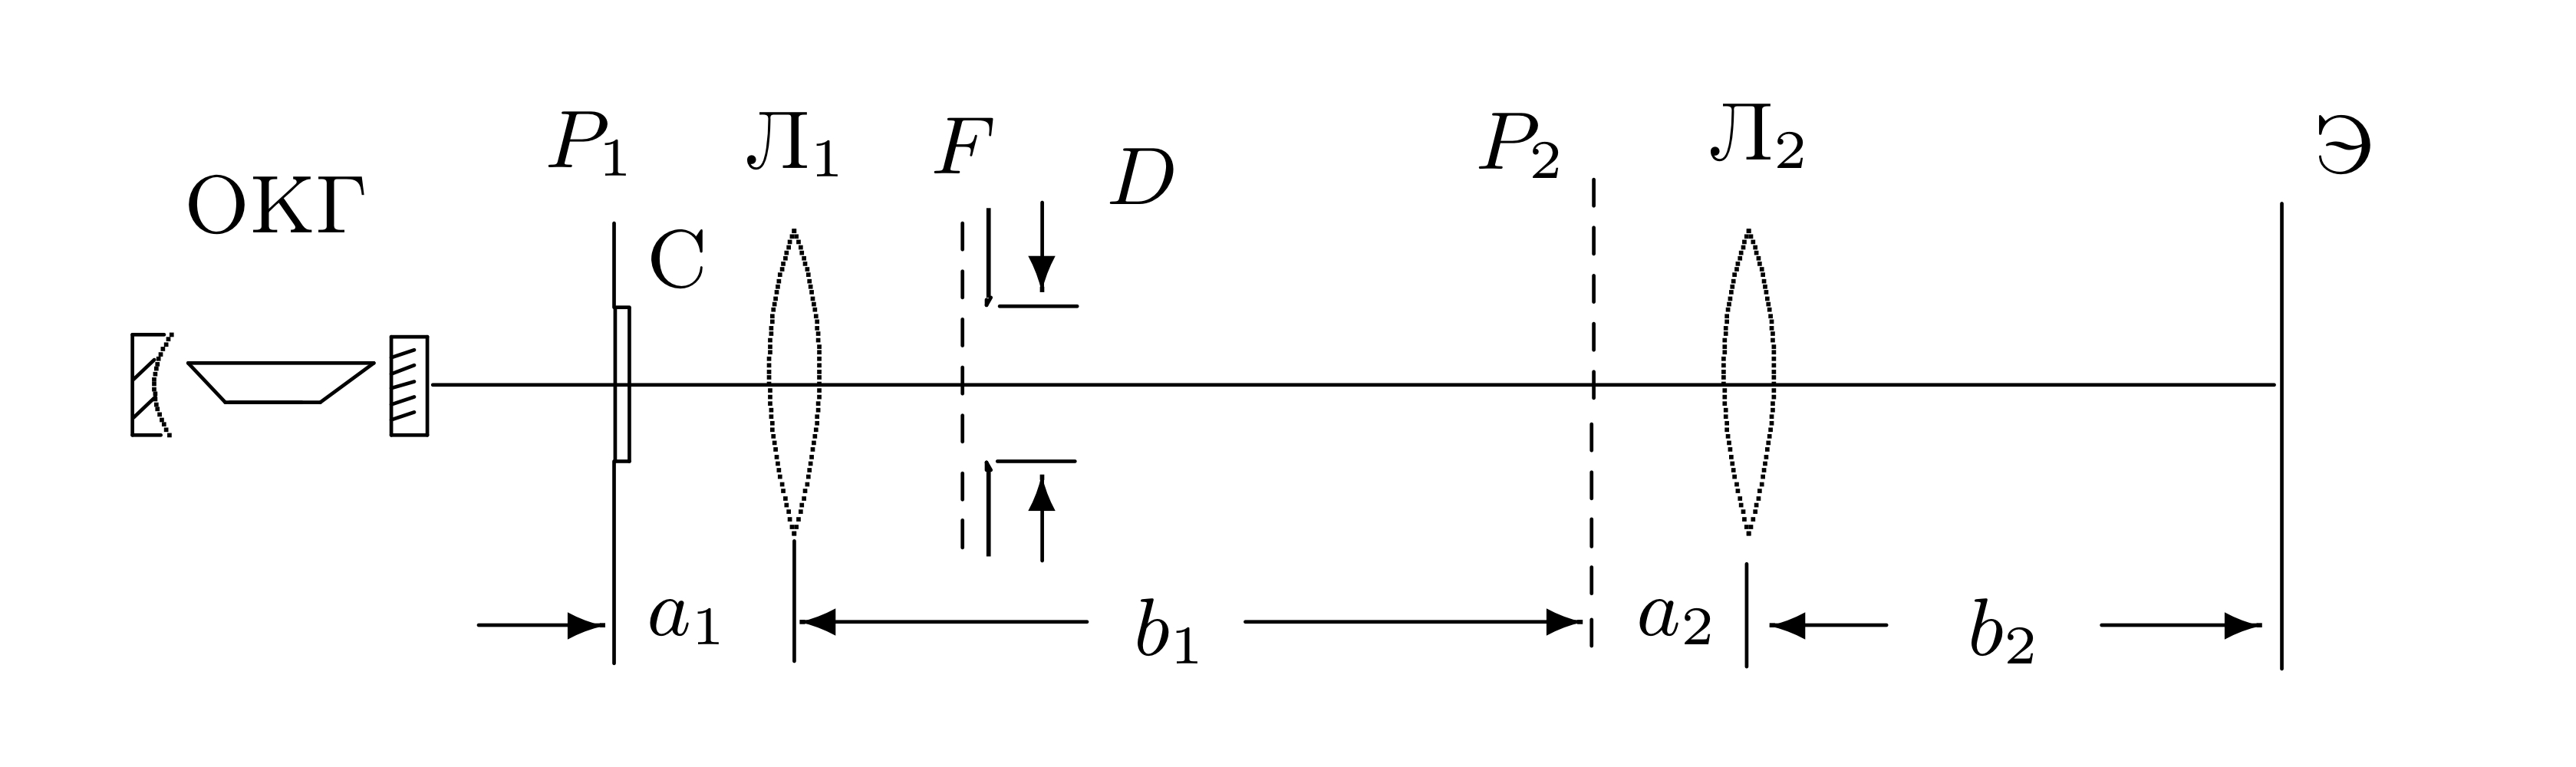
\includegraphics[scale=0.14]{4.3.3/micro.jpeg}
    \caption{Схема экспериментальной установки — модель проекционного микроскопа}
    \label{micro}
\end{figure}

Излучение лазера (ОКГ) почти перпендикулярно падает на сетку С, установленную вблизи фокальной плоскости линзы Л$_1$ -- объектива микроскопа. Обычно и объектив, и окуляр микроскопа -- короткофокусные линзы (1–3 см). В нашей модели линза Л$_1$ выбирается достаточно длиннофокусной ($f \approx 10$ см), т. к. размер первичного изображения в фокальной плоскости $F$ должен быть не слишком малым, чтобы дополнительными диафрагмами можно было влиять на вторичное изображение в плоскости $P_2$. Вторичное изображение из плоскости $P_2$ проецируется на экран Э линзой Л$_2$ (короткофокусной, чтобы изображение на экране было крупнее). Во избежание микротравм глаза от излучения лазера не следует использовать эту линзу традиционным образом как окуляр микроскопа.
Изображение сетки периодически повторяется -- \textit{репродуцируется} -- в пространстве между сеткой и первой линзой, поэтому для того, чтобы среди множества репродуцированных изображений сетки можно было выделить её геометрическое изображение, на сетках изображён лисёнок, т. е. непериодический объект, изображение которого не репродуцируется.
В фокальной плоскости $F$ могут быть установлены диафрагмы — щелевая или ирисовая (отверстие с переменным диаметром) и различного рода маски (препятствия).
Как видно из соотношения \eqref{diaf}, минимально разрешимый шаг решётки или сетки определяется апертурным углом A объектива. Обычно апертура микроскопа меняется при помощи ирисовой диафрагмы на объективе (на линзе Л$_1$ такая диафрагма есть), но в наших условиях удобнее располагать щелевую диафрагму в плоскости $F$. Имея набор сеток с различными периодами $d$ и изменяя апертурный угол объектива с помощью щелевой диафрагмы, можно экспериментально проверить соотношение \eqref{diaf}.

\section{Ход работы и обработка результатов}

\subsection{Определение периодов решеток по дифракционной картине}

В нашей работе период сеток рассчитывается двумя способами: в первом способе (по дифракции Фраунгофера) расстояние между дифракционными максимумами на экране измеряется при помощи линейки, а затем по формулам \eqref{max} определяется её период; во втором способе период определяется по увеличенному (с помощью модели микроскопа) изображению сетки на экране.

Длина волны лазера $\lambda = 532$ нм; расстояние между решеткой и экраном $H = 143\pm 1$см.

\floatsetup[table]{capposition=top}

\begin{table}[H]
    \centering
    \begin{tabular}{|p{2cm}|l|p{2cm}|l|l|}
        \hline N\textsuperscript{\underline{o}} реш. & $\Delta m$ & $l$, мм & $\displaystyle d= \Delta m \lambda H/l$, мкм & $\varepsilon_d$, \% \\ \hline
         1&2 & 152 & 10,0 & 1,4 \\ \hline
         2&8 & 248 & 24,5 & 1,1 \\ \hline
         3&16& 245 & 49,7 & 1,1 \\ \hline
    \end{tabular}
    \caption{Периоды дифракционных решеток}
    \label{d}
\end{table}

\subsection{Определение периодов решеток по увеличенному изображению}

Данные оптической системы представлены ниже (все значения в см, увеличение безразмерное):

\begin{center}
    $
    F_1 = 11; \ \ \ F_2 = 2,5;\\
    a_1 = 13,5 \pm 0,2; \ \ \ a_2 \approx F_2;\\
    b_1 = 58,0 \pm 0,2; \ \ \ b_2 = 68,5 \pm 0,2;\\
    \Gamma = b_1 b_2/(a_1 a_2) = 117,7 \pm 2,5
    $
\end{center}

Полученные данные приведены в таблице \ref{d'}.

\begin{table}[H]
    \centering
    \begin{tabular}{|p{2cm}|l|p{2cm}|l|l|}
        \hline N\textsuperscript{\underline{o}} реш. & $\Delta m$ & $l$, мм & $\displaystyle d= l/\Delta m\Gamma$, мкм & $\varepsilon_d$, \% \\ \hline
        1& 30 & 38 & 10,8 & 3,4 \\ \hline
        2& 12 & 37 & 26,2 & 3,5 \\ \hline
        3& 15 & 95 & 53,8 & 2,7 \\ \hline
    \end{tabular}
    \caption{Периоды дифракционных решеток}
    \label{d'}
\end{table}

\subsection{Определение разрешающей способности микроскопа}

С помощью откалиброванных таким образом сеток определяется разрешающая способность микроскопа. Для этого в задней фокальной плоскости $F$ объектива устанавливается щелевая диафрагма с микрометрическим винтом и подбирается её минимальный размер, при котором ещё видно изображение сетки на экране (щель пропускает максимумы с $m = 0, \pm 1$). По размеру диафрагмы и фокусному расстоянию объектива рассчитывается апертурный угол $u$ и проверяется соотношение \eqref{diaf}.

Измерения приведены в таблице \ref{D}.

\begin{table}[H]
    \centering
    \begin{tabular}{|p{2cm}|p{2cm}|p{2cm}|p{2cm}|p{2cm}|}
        \hline N\textsuperscript{\underline{o}} реш. & $D$, мм & $d_{\text{эксп}}$, мкм & $\varepsilon_{d_{\text{эксп}}}$, \% & $d_{\text{теор}}$, мкм \\ \hline
        1& >4   & <29  & <1,2& 10 \\ \hline
        2& 2,21 & 53   & 2,2 & 25 \\ \hline
        3& 1,03 & 114  & 4,9 & 50 \\ \hline
        
    \end{tabular}
    \caption{Минимальное расстояние, разрешаемое микроскопом}
    \label{D}
\end{table}

По полученным (не лучшим) данным, был построен график на рис. \ref{gr}.

\begin{figure}[H]
    \centering
    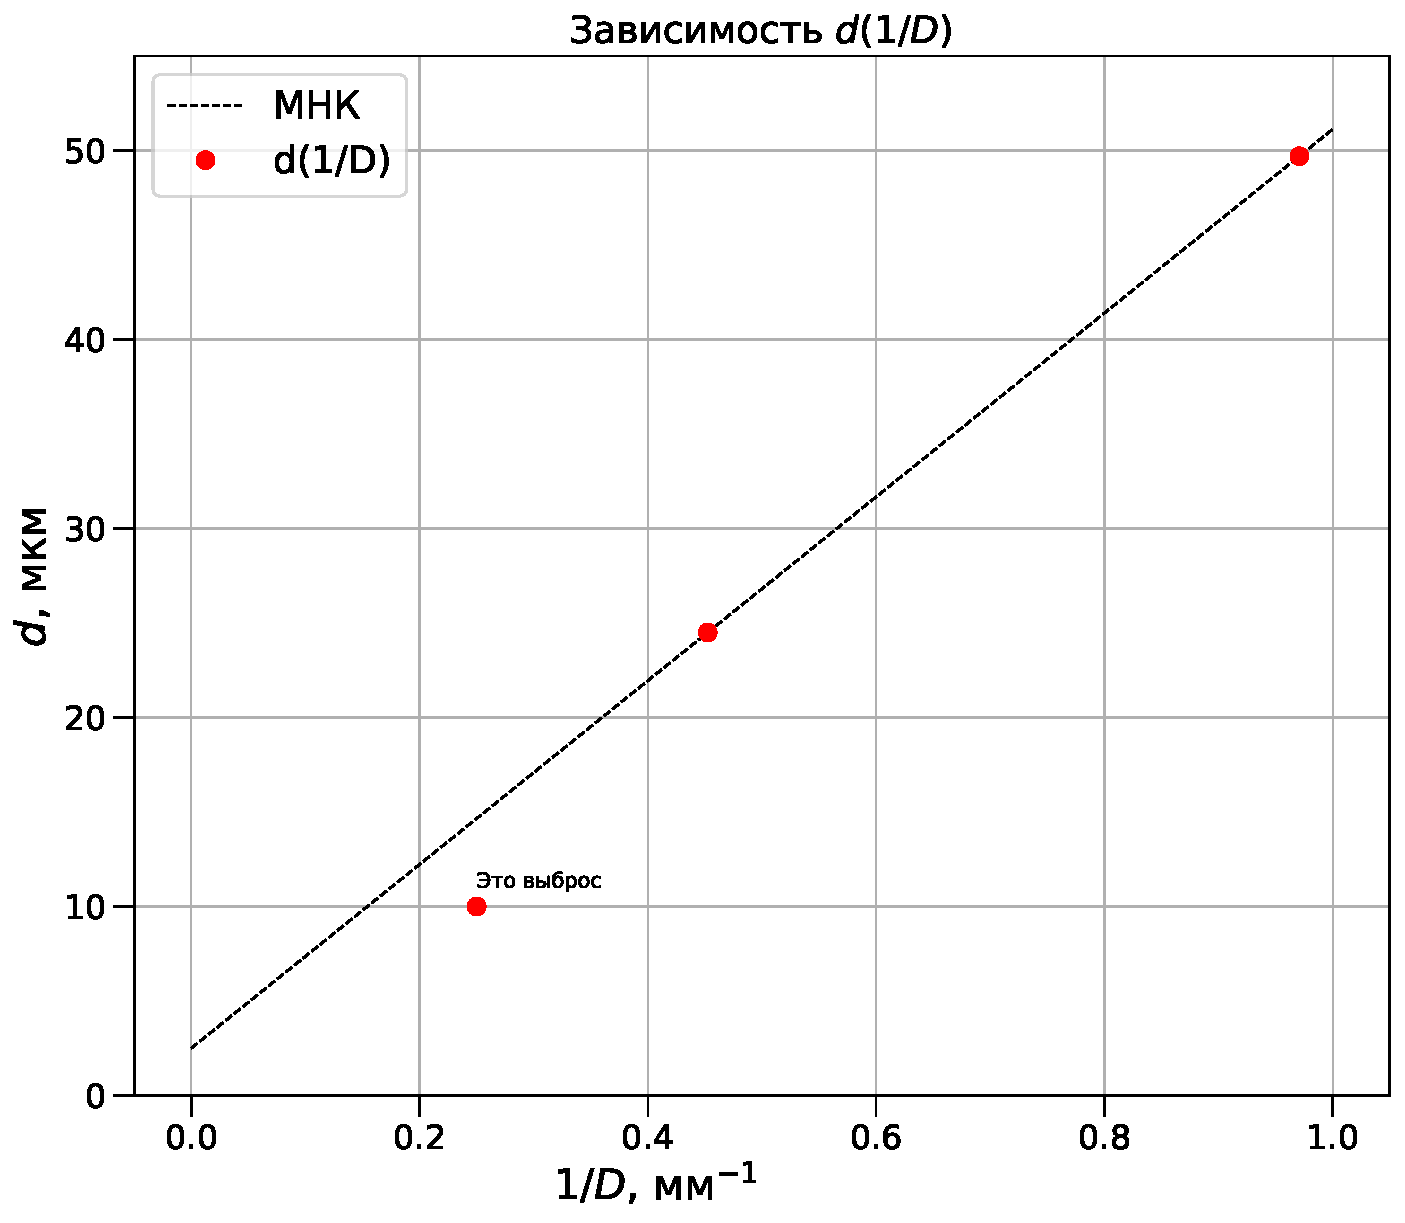
\includegraphics[scale=0.65]{4.3.3/d.pdf}
    \caption{График зависимости $d(1/D)$}
    \label{gr}
\end{figure}

По полученным данным сложно что-либо сказать о справедливости теории Аббе. Есть необходимость проделать более точные измерения (выброс на графике обусловлен органицением шкалы микрометра).

\subsection{Пространственная фильтрация и мультиплицирование}

В процессе проведения опытов по пространственной фильтрации и мультиплицированию были получены следющие фотографии (см. раздел "Приложение").






\section{Вывод}


По измерениям спектров получилось определить дифракционные углы и по теоретическим формулам рассчитать периоды решеток. Полученные данные сошлись с результатами,  полученными по измерениям увеличенных с помощью микроскопа изображений сеток.


\section{Приложение}

\end{document}
